\section{Current sequential approach}

\begin{frame}{Note: No neighbour SPs}
SPs with no neighbours are uninteresting from a computing perspective (a priori).

\begin{itemize}
\item They can be resolved with a mere lookup ($2^8 = 256$ possibilities)
\item There is no guarantee there will be FPGA resources to activate this bit
\end{itemize}
\end{frame}

\begin{frame}{SPs with neighbours}
The current implementation computes every sensor independently from each other:

\begin{itemize}
\item Prepare an array of $768 * 256$ booleans
\item Add every SP with neighbours to the array
\item Add every active pixel as a \emph{candidate}
\item Traverse candidates using a BFS algorithm, zeroing visited pixels in the array
\end{itemize}
\end{frame}

\begin{frame}{Sequential algorithm (1)}
\begin{center}
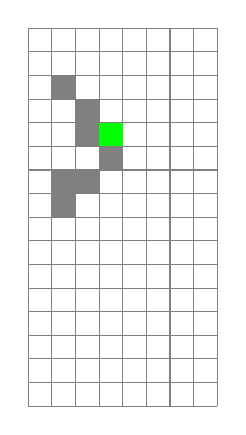
\begin{tikzpicture}[x=3mm, y=3mm]
% Grid
\draw[step=3mm,gray,thin] (0,0) grid (8,16);

% Pixels
\fill[gray] (2,12) rectangle (3,13);
\fill[gray] (2,11) rectangle (3,12);
\fill[gray] (2,9) rectangle (3,10);
\fill[green] (3,11) rectangle (4,12);
\fill[gray] (3,10) rectangle (4,11);
\fill[gray] (1,13) rectangle (2,14);
\fill[gray] (1,9) rectangle (2,10);
\fill[gray] (1,8) rectangle (2,9);
\end{tikzpicture}
\end{center}
\end{frame}

\begin{frame}{Sequential algorithm (2)}
\begin{center}
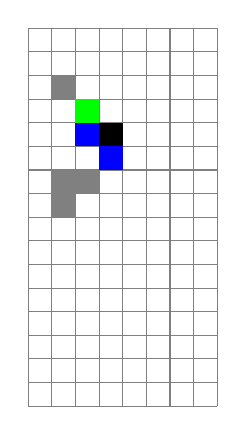
\begin{tikzpicture}[x=3mm, y=3mm]
% Grid
\draw[step=3mm,gray,thin] (0,0) grid (8,16);

% Pixels
\fill[gray] (2,9) rectangle (3,10);
\fill[gray] (1,13) rectangle (2,14);
\fill[gray] (1,9) rectangle (2,10);
\fill[gray] (1,8) rectangle (2,9);

% Forming cluster
\fill[black] (3,11) rectangle (4,12);
\fill[green] (2,12) rectangle (3,13);
\fill[blue] (2,11) rectangle (3,12);
\fill[blue] (3,10) rectangle (4,11);
\end{tikzpicture}
\end{center}
\end{frame}

\begin{frame}{Sequential algorithm (3)}
\begin{center}
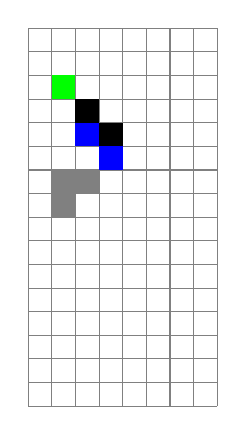
\begin{tikzpicture}[x=3mm, y=3mm]
% Grid
\draw[step=3mm,gray,thin] (0,0) grid (8,16);

% Pixels
\fill[gray] (1,9) rectangle (2,10);
\fill[gray] (1,8) rectangle (2,9);
\fill[gray] (2,9) rectangle (3,10);

% Forming cluster
\fill[black] (3,11) rectangle (4,12);
\fill[black] (2,12) rectangle (3,13);
\fill[green] (1,13) rectangle (2,14);
\fill[blue] (2,11) rectangle (3,12);
\fill[blue] (3,10) rectangle (4,11);
\end{tikzpicture}
\end{center}
\end{frame}

\begin{frame}{Sequential algorithm (4)}
\begin{center}
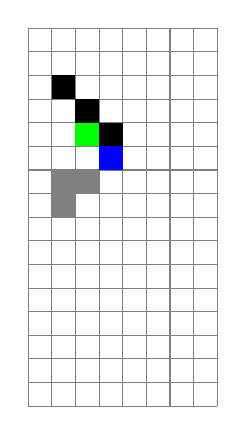
\begin{tikzpicture}[x=3mm, y=3mm]
% Grid
\draw[step=3mm,gray,thin] (0,0) grid (8,16);

% Pixels
\fill[gray] (1,9) rectangle (2,10);
\fill[gray] (1,8) rectangle (2,9);
\fill[gray] (2,9) rectangle (3,10);

% Forming cluster
\fill[black] (3,11) rectangle (4,12);
\fill[black] (2,12) rectangle (3,13);
\fill[black] (1,13) rectangle (2,14);
\fill[green] (2,11) rectangle (3,12);
\fill[blue] (3,10) rectangle (4,11);
\end{tikzpicture}
\end{center}
\end{frame}

\begin{frame}{Performance}
Out of the 16.39~\% in the image:

\vspace{-10pt}
\begin{itemize}
\item 6~\% is sorting
\item 5~\% is dealing with no-neighbouring SPs
\item The described algorithm takes 5~\% of the full HLT1 sequence
\end{itemize}

\begin{figure}
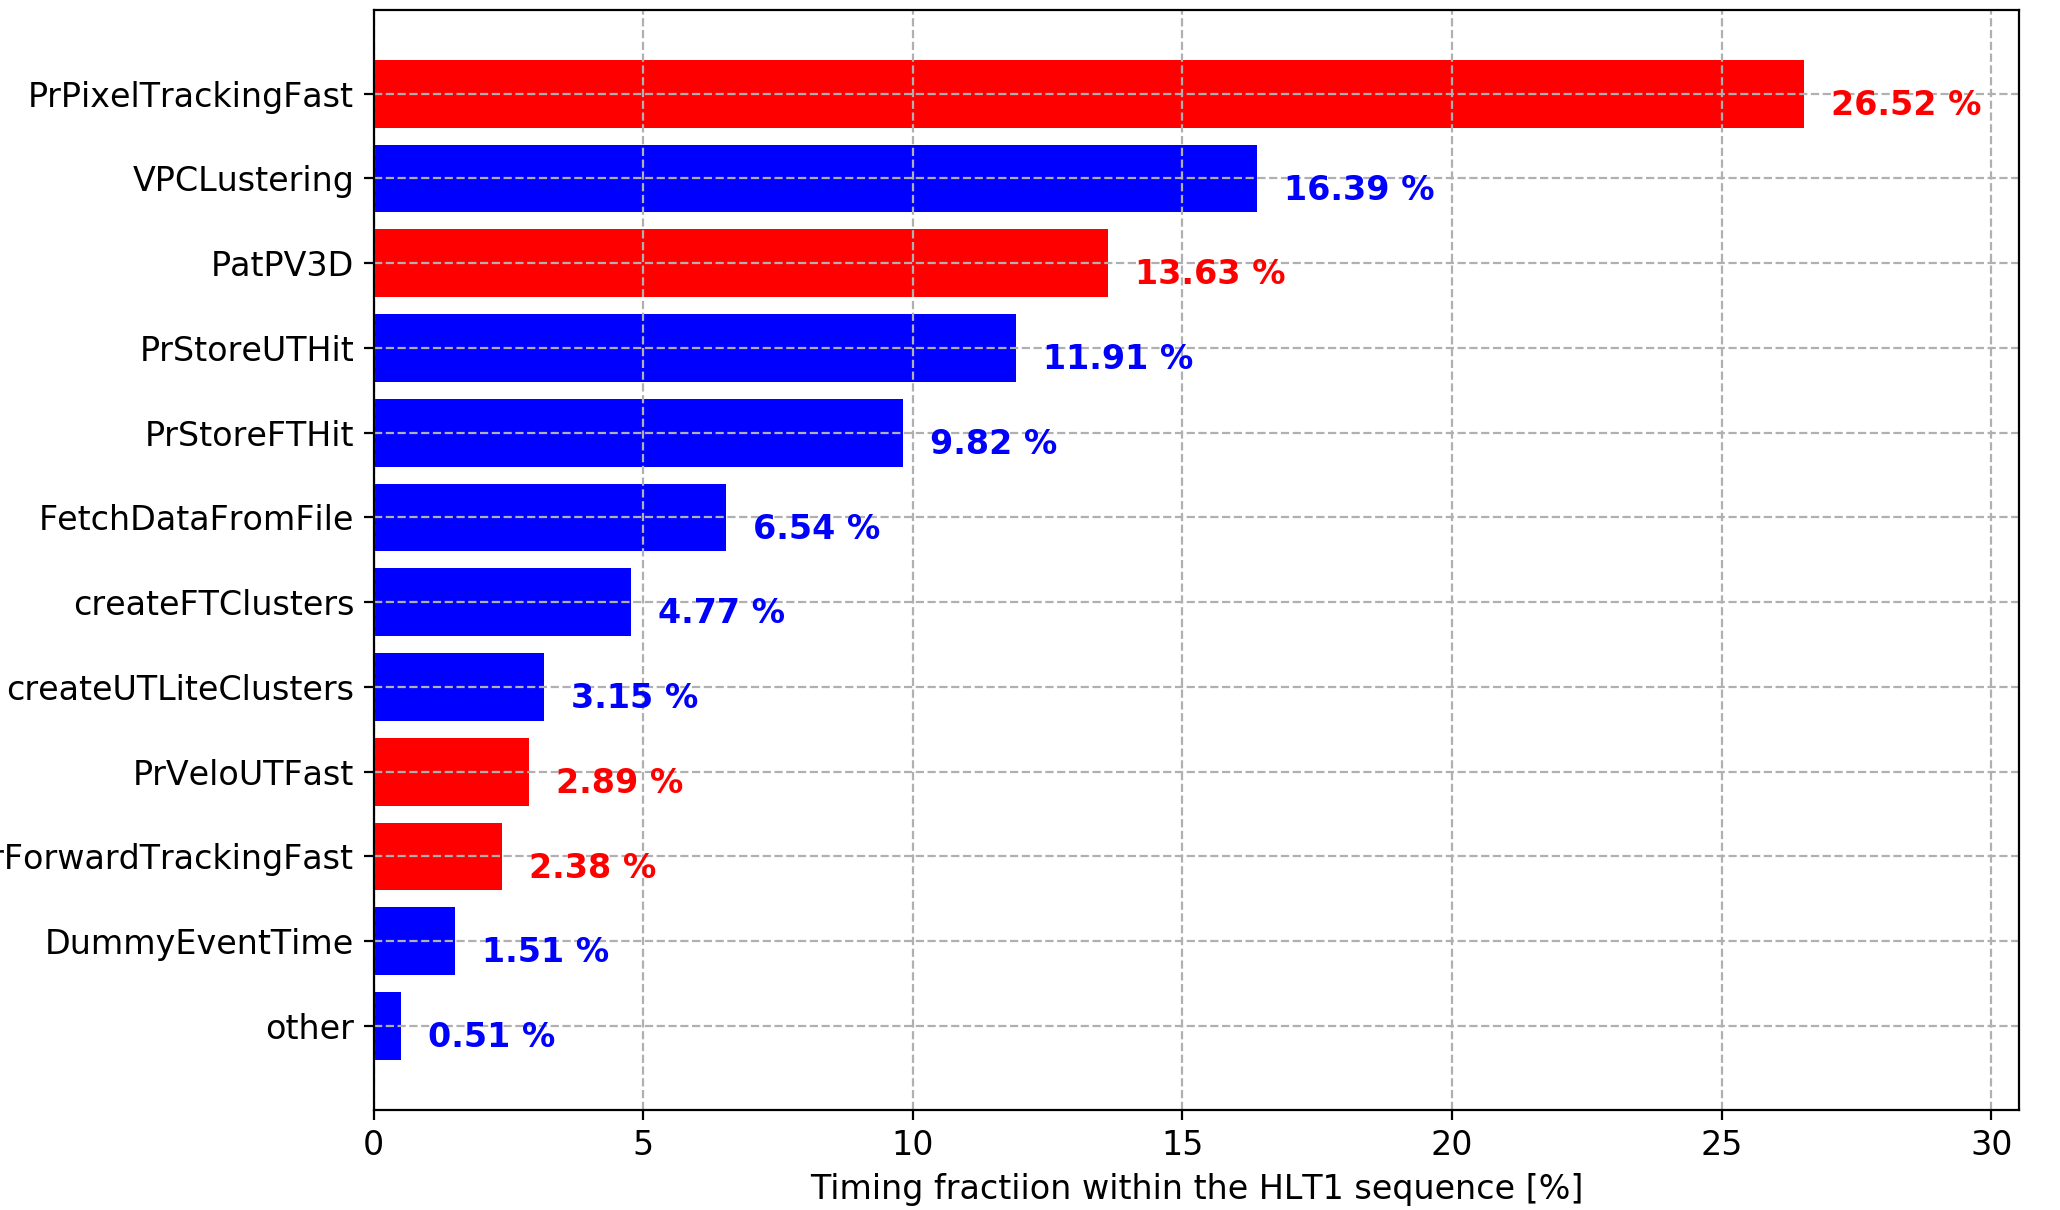
\includegraphics[width=0.5\textwidth]{hlt_sequence_distribution}
\end{figure}
\end{frame}

\begin{frame}{Caveats for parallelization}
I would argue the current algorithm is rather fast and \emph{deeply} sequential:

\begin{itemize}
\item Relies on an array describing the whole sensor
\item Imposes a RAW in the processing of candidates
\item Populates each module incrementally, relies on raw banks being ordered
\end{itemize}
\end{frame}

\begin{frame}{Additional caveats for GPUs}
GPUs are especially bad for incremental datatypes.

\begin{itemize}
\item Datatype sizes should be known a priori, in order to avoid too much \emph{over provisioning} and copying
\item Holding the full event (5~MB per event) is too memory-hungry
\end{itemize}

In order to have an efficient GPU algorithm, we need:

\begin{itemize}
\item A fast way to estimate the memory required. Underestimating is not acceptable, but overestimating by a \emph{little bit} would be ok.
\item A local algorithm to perform clustering that does not require the full sensor laid down, maintaining code branching low.
\item Note: Finding the real clusters is desirable, but a good approximation is also ok.
\end{itemize}
\end{frame}
